% Use a modern class instead of an old article class
\documentclass{scrartcl}

% The class "scrartcl" provides the “article”-like element of the koma-script collection. The document layout of the class is less 'strident' than that of article, and it offers much more flexibility than article via other elements of the koma-script collection.

% Information about other document classes can be found herehttps://en.wikibooks.org/wiki/LaTeX/Document_Structure#Document_classes


% %%%%%%%%%%%%%%%%%%%%%%%%%%% CUSTOM PACKAGES %%%%%%%%%%%%%%%%%%%%%%%%%%% %
\usepackage[none]{hyphenat}
% \usepackage{geometry}
\usepackage{float}
\usepackage{amssymb}
\usepackage{amsthm}
\usepackage{empheq}
\usepackage{mdframed}
\usepackage{lipsum}
\usepackage{color}
\usepackage{bm}
\usepackage{array}
\usepackage{enumitem}
\usepackage{subfigure}
\usepackage[most]{tcolorbox}
\usepackage{soul}

\usepackage[a4paper, left=2cm, right=2cm]{geometry}

% Long table
\usepackage{xltabular}

%maths
\usepackage{amsfonts}

\usepackage[edges]{forest}
\usepackage[T1]{fontenc}

%tikzpicture
\usepackage{tikz}
\usepackage{scalerel}
\usepackage{tkz-euclide}
\usetikzlibrary{trees}
\usetikzlibrary{calc}
\usetikzlibrary{patterns,arrows.meta}
\usetikzlibrary{shadows}
\usetikzlibrary{external}
\usepackage{tikz-cd}


%pgfplots
\usepackage{pgfplots}  % For plots and graphs
\usepgfplotslibrary{statistics}
\usepgfplotslibrary{fillbetween}

% \usepackage{cellspace} % Adds extra space inside table cells
% \setlength\cellspacetoplimit{12px}    % Top padding
% \setlength\cellspacebottomlimit{12px} % Bottom padding

\renewcommand{\arraystretch}{1.5} % Increase row height (default = 1.0)
\usepackage{tabularx}
% Define a new column type: vertically centered and flexible width
\newcolumntype{M}[1]{>{\centering\arraybackslash}m{#1}}
\newcolumntype{Y}{>{\centering\arraybackslash}X} % Like M but auto width
% %%%%%%%%%%%%%%%%%%%%%%%%%%% CUSTOM PACKAGES %%%%%%%%%%%%%%%%%%%%%%%%%%% %
% %%%%%%%%%%%%%%%%%%%%%%%%%%% CUSTOM COMMANDS %%%%%%%%%%%%%%%%%%%%%%%%%%% %
% \usepackage{tocbasic}
% \DeclareNewSectionCommand[
%   level=4,
%   indent=0pt,
%   beforeskip=1.5ex plus .2ex minus .1ex,
%   afterskip=.8ex plus .2ex,
%   style=section,
%   font=\normalfont\normalsize\bfseries
% ]{subsubsubsection}

% % TOC depth and numbering depth
% \setcounter{tocdepth}{4}
% \setcounter{secnumdepth}{4}

% % Adjust indentation in TOC
% \DeclareTOCStyleEntry[
%   indent=1.5em,
%   numwidth=3em
% ]{tocline}{subsubsubsection}

% Extend sectioning to level 4 (subsubsubsection)
\makeatletter
\newcounter{subsubsubsection}[subsubsection]
\renewcommand\thesubsubsubsection{\thesubsubsection.\arabic{subsubsubsection}}

\newcommand\subsubsubsection{\@startsection{subsubsubsection}{4}{\z@}%
  {-3.25ex \@plus -1ex \@minus -.2ex}%
  {1.5ex \@plus .2ex}%
  {\normalfont\normalsize\bfseries}}

\newcommand\l@subsubsubsection{\@dottedtocline{4}{5em}{4em}}
\makeatother

% Add subsubsubsection to TOC and numbering
\setcounter{secnumdepth}{4}
\setcounter{tocdepth}{4}

% %%%%%%%%%%%%%%%%%%%%%%%%%%% CUSTOM COMMANDS %%%%%%%%%%%%%%%%%%%%%%%%%%% %
% --------------------------- DEFAULT PACKAGES SETUP --------------------------- %
\usepackage[utf8]{inputenc} % Specify the input encoding of the source file as UTF8 
\usepackage[T1]{fontenc} % The T1 font encoding is an 8-bit encoding and fully supports words containing accented characters
\usepackage{lmodern} % Load Latin modern fonts in outline format
\usepackage{inconsolata} % Load better typewriter font
\usepackage[english]{babel} % For better hyphenation patterns
\usepackage{microtype} % For improved micro-typography
\frenchspacing % Switch off extra space after a sentence
\usepackage{graphicx} % To be able to iclude pictures
\usepackage{mathtools,amsmath} % for advanced math formulas
\usepackage{minted} % To highlight source code
% Default options for all minted environments
\setminted{
    style=default, % for minted envronment
    autogobble, % automatically remove all common leading whitespace
    xleftmargin=10pt, % indentation to add (on the left) before the listing
    numbersep=6pt, % gap between numbers and start of line
    linenos, % enables line numbers
    mathescape % enables the usual math mode inside comments
}
\setmintedinline[c]{style=default} % for minted inlines
\usepackage{fancyvrb} % Flexible handling of verbatim text
\usepackage{booktabs} % For well-spaced lines and guidelines in tables
\usepackage{algorithm} % To typeset algorithms or pseudocode in LaTeX 
\usepackage{algpseudocode}
\pgfplotsset{width=10cm,compat=1.9}
\renewcommand{\algorithmiccomment}[1]{\hspace{1cm}// #1}

\usepackage{soul} % Change text highlighting
\usepackage{pgffor} % Needed for for-loops

% --------------------------- DEFAULT PACKAGES SETUP --------------------------- %
% --------------------------- KOMA OPTIONS (DOCUMENT SETTINGS) ----------------------- %

\KOMAoptions{
    parskip=half,  % full, off
    fontsize=12pt, % base font size (10pt default)
    toc=sectionentrydotfill, % Fill toc with dots for sections
    % headings=big,% small/normal/big headings (normal is default), 
    % paper=a5,    % paper format (a4 default) 
    pagesize=auto  % Use paper format for PDF too
}

% --------------------------- KOMA OPTIONS (DOCUMENT SETTINGS) ----------------------- %
%%%%%%%%%%%%%%%%%%%%%%%%%% Define some useful colors %%%%%%%%%%%%%%%%%%%%%%%%%%
\definecolor{ocre}{RGB}{243,102,25}
\definecolor{mygray}{RGB}{243,243,244}
\definecolor{deepGreen}{RGB}{26,111,0}
\definecolor{shallowGreen}{RGB}{235,255,255}
\definecolor{deepBlue}{RGB}{61,124,222}
\definecolor{shallowBlue}{RGB}{235,249,255}
%%%%%%%%%%%%%%%%%%%%%%%%%%%%%%%%%%%%%%%%%%%%%%%%%%%%%%%%%%%%%%%%%%%%%%%%%%%%%%%

%%%%%%%%%%%%%%%%%%%%%%%%%% Define an orangebox command %%%%%%%%%%%%%%%%%%%%%%%%
\newcommand\orangebox[1]{\fcolorbox{ocre}{mygray}{\hspace{1em}#1\hspace{1em}}}
%%%%%%%%%%%%%%%%%%%%%%%%%%%%%%%%%%%%%%%%%%%%%%%%%%%%%%%%%%%%%%%%%%%%%%%%%%%%%%%

%%%%%%%%%%%%%%%%%%%%%%%%%%%% English Environments %%%%%%%%%%%%%%%%%%%%%%%%%%%%%
\newtheoremstyle{mytheoremstyle}{3pt}{3pt}{\normalfont}{0cm}{\rmfamily\bfseries}{}{1em}{{\color{black}\thmname{#1}~\thmnumber{#2}}\thmnote{\,--\,#3}}
\newtheoremstyle{myproblemstyle}{3pt}{3pt}{\normalfont}{0cm}{\rmfamily\bfseries}{}{1em}{{\color{black}\thmname{#1}~\thmnumber{#2}}\thmnote{\,--\,#3}}
\theoremstyle{mytheoremstyle}
\newmdtheoremenv[linewidth=1pt,backgroundcolor=shallowGreen,linecolor=deepGreen,leftmargin=0pt,innerleftmargin=20pt,innerrightmargin=20pt,]{theorem}{Theorem}[section]
\theoremstyle{mytheoremstyle}
\newmdtheoremenv[linewidth=1pt,backgroundcolor=shallowBlue,linecolor=deepBlue,leftmargin=0pt,innerleftmargin=20pt,innerrightmargin=20pt,]{definition}{Definition}[section]
\theoremstyle{myproblemstyle}
\newmdtheoremenv[linecolor=black,leftmargin=0pt,innerleftmargin=10pt,innerrightmargin=10pt,]{problem}{Problem}[section]
%%%%%%%%%%%%%%%%%%%%%%%%%%%%%%%%%%%%%%%%%%%%%%%%%%%%%%%%%%%%%%%%%%%%%%%%%%%%%%%

%%%%%%%%%%%%%%%%%%%%%%%%%%%%%%% Plotting Settings %%%%%%%%%%%%%%%%%%%%%%%%%%%%%
\usepgfplotslibrary{colorbrewer}
\pgfplotsset{width=8cm,compat=1.9}
%%%%%%%%%%%%%%%%%%%%%%%%%%%%%%%%%%%%%%%%%%%%%%%%%%%%%%%%%%%%%%%%%%%%%%%%%%%%%%%
% %%%%%%%%%%%%%%%%%%%%%%%%%%%%%%%%%%%%%% REPORT DETAILS %%%%%%%%%%%%%%%%%%%%%%%%%%%%%% %

\newcommand{\courseyear}{2026}
\newcommand{\coursename}{TFSS25 - Reinforcement Learning}
\newcommand{\coursecredits}{7.5 credits}
\newcommand{\fullcoursename}{\coursename, \coursecredits}
\newcommand{\termname}{Autumn\courseyear}
% \newcommand{\groupnumber}{10} % Optional
\newcommand{\reportname}{Reinforcement Learning Project Report}
\newcommand{\assignmentname}{Reinforcement Learning}

% %%%%%%%%%%%%%%%%%%%%%%%%%%%%%%%%%% REPORT DETAILS %%%%%%%%%%%%%%%%%%%%%%%%%%%%%%%%%% %
% -------------------------- SETTING UP PROPERTIES OF PDF FILE ----------------------- %

\usepackage{hyperref}
\usepackage[all]{hypcap}
\hypersetup{
    colorlinks=true,
    allcolors=blue,
    pdftitle={\reportname},
    pdfauthor={Martin Nilsson},
    pdfsubject={\coursename, \termname}
	% pdfpagemode=FullScreen,
	% pdfpagemode= UseOutlines % the default if present
}

% ---------------------------- SETTING UP PROPERTIES OF PDF FILE ------------------------ %
% ----------------------------- HEADER AND FOOTER SETTINGS ------------------------------ %

\usepackage{scrlayer-scrpage}
\usepackage{zref-totpages} % To get the total number of pages
\pagestyle{scrheadings}
\KOMAoptions{% 
    headsepline,% line below the header
    plainheadsepline,% also on scrplain
}
\clearscrheadfoot % Erase all current configurations
% inner part of the header [titel_page]{other_pages}
\ihead[\coursename, \courseyear]{\coursename, \courseyear}
% outer part of the header [titel_page]{other_pages}
\ohead{\assignmentname}
% center part of the footer [titel_page]{other_pages}
\cfoot[\textup{Page \pagemark\ of \ztotpages}]{\textup{Page \pagemark\ of \ztotpages}}

% ----------------------------- HEADER AND FOOTER SETTINGS ------------------------------ %
% %%%%%%%%%%%%%%%%%%%%%%%%%%%%%%%%%% TITLE PAGE CONFIG %%%%%%%%%%%%%%%%%%%%%%%%%%%%%%%%%% %

\title{\reportname}
\subtitle{Snow plow problem with multi-agent reinforcement learning}
\author{
    \textbf{Authors:} \\
    \textbf{Martin Nilsson}, \textit{School of Engineering}, Jönköping University
    \and
    \textbf{Besan Ewir}, \textit{School of Engineering}, Jönköping University
    \and
    \textbf{Vladimir Giustacchini}, \textit{School of Engineering}, Jönköping University
    \and
    \textbf{Jorge Cuello}, \textit{School of Engineering}, Jönköping University
}
\date{\today}

% %%%%%%%%%%%%%%%%%%%%%%%%%%%%%%%%%% TITLE PAGE CONFIG %%%%%%%%%%%%%%%%%%%%%%%%%%%%%%%%%% %


\begin{document} % <<<<<<<<<<<<<<<<<<<<<<<<<<<<<<<<<<<<<<<<<<<<<<
\raggedright

\maketitle

\tableofcontents

\newpage

\section{Problem Description: Snow Plow Problem}

We consider a snow plow problem where a single or group of snow plows is tasked with clearing snow from a network of roads in a city. The objective is to \st{minimize the total time taken to clear all roads while ensuring that the snow plows operate efficiently and avoid collisions}. Each snow plow is controlled by an agent that makes decisions based on the current state of the environment, including the location of other snow plows, the amount of snow on each road, and the traffic conditions.

\section{Environment}

A grid represents the city, where each cell corresponds to a road segment. The state of the environment includes the positions of all snow plows, the amount of snow on each road segment, and any obstacles or traffic conditions that may affect the movement of the snow plows.

\subsection{Rules}

The snow plows can move in four directions (UP, DOWN, LEFT, RIGHT) and can also choose to stay in their current position (DO\_NOTHING). The environment is dynamic in the sense that snow randomly falls onto road cells in the grid environment periodically based on a \verb|cloud_prob| $= 0.02$ $\times$ \verb|number_of_agents|. This is only to balanced the snow level accumulation to give the snow plows a fair difficulty across different map sizes and number of agents. and the agents must adapt their strategies accordingly.

To enforce cooperative behavior, we introduced additional rules to the environment that lets multiple agents to collaborate with snow cells with \verb|snow_level| $> 1$. So agents placed in the same grid cell that faces the same snow cell will have reduced time to clear the snow compared to doing it alone and would therefore clear snow and earn rewards faster. See table \ref{tab:single_plow_time} for more information.

\begin{table}[H]
    \begin{minipage}{.5\linewidth}
        \centering
        \begin{tabular}{|c|c|}
            \hline
            \texttt{Snow\_level} & \textbf{Time steps} \\
            \hline
            3                    & 10                  \\
            \hline
            2                    & 5                   \\
            \hline
            1                    & 1                   \\
            \hline
        \end{tabular}
        \caption{Single agent plow times}
        \label{tab:single_plow_time}
    \end{minipage}
    \begin{minipage}{.5\linewidth}
        \centering
        \begin{tabular}{|c|c|}
            \hline
            \texttt{Snow\_level} & \textbf{\textcolor{red}{Time steps}} \\
            \hline
            3                    & 6                                    \\
            \hline
            2                    & 3                                    \\
            \hline
            1                    & 1                                    \\
            \hline
        \end{tabular}
        \caption{Multi-agent plow times}
        \label{tab:multi_plow_time}
    \end{minipage}
\end{table}

\subsubsection{Traffic rules}

The agents cannot navigate the road network however they want. There are traffic rules applied for each type of grid cells that they need to follow. The environment is initialized with the intended traffic rules for each grid cell. Different rules will apply depending on the cell type and remove invalid actions that would make the agents disobey traffic rules, go into obstacle cells or attempt to go outside of the grid area for different traffic situations.

The types are as follows:

\begin{table}[H]
    \centering
    \begin{tabularx}{\textwidth}{|Y|Y|M{0.5\textwidth}|}
        \hline
        \textbf{Cell type}
         & \textbf{Color}
         & \textbf{Traffic rules}                                                                      \\\hline
        ROAD
         & Grey
         & Any direction is allowed.                                                                   \\\hline
        HIGHWAY
         & Light Grey
         & One way direction only.                                                                     \\\hline
        INTERSECTION
         & Dark Grey
         & Remove the action that normally would lead back to going in the opposite highway direction. \\\hline
    \end{tabularx}
    \caption{Road Network Grid Cell Types}
    \label{tab:road_cells}
\end{table}

\subsection{Actions}

\begin{enumerate}
    \item $\rightarrow$: Move Right
    \item $\leftarrow$: Move Left
    \item $\uparrow$: Move Up
    \item $\downarrow$: Move Down
    \item Do nothing: Stay in the current position.
\end{enumerate}

\subsection{Observations}


\begin{table}[H]
    % \begin{minipage}{.5\linewidth}
    %     \centering
    %     \begin{tabular}{|c|c|}
    %         \hline
    %         \textbf{Field} & \textbf{Description} \\
    %         \hline
    %         \texttt{grid}  & -                    \\
    %         \hline
    %         \texttt{agent\_positions}  & -                    \\
    %         \hline
    %         \texttt{self\_position}  & -                    \\
    %         \hline
    %         \texttt{grid}  & -                    \\
    %         \hline
    %         \texttt{grid}  & -                    \\
    %         \hline
    %         \texttt{grid}  & -                    \\
    %         \hline
    %     \end{tabular}
    %     \caption{Full Observability}
    %     \label{tab:first}
    % \end{minipage}%
    % \begin{minipage}{.5\linewidth}
    \centering
    \begin{tabular}{|c|c|}
        \hline
        \textbf{Field}            & \textbf{Description} \\
        \hline
        \texttt{grid}             & -                    \\
        \hline
        \texttt{agent\_positions} & -                    \\
        \hline
        \texttt{self\_position}   & -                    \\
        \hline
        \texttt{self\_id}         & -                    \\
        \hline
        \texttt{view\_origin}     & -                    \\
        \hline
    \end{tabular}
    \caption{Full and Partial Observability parameters}
    \label{tab:obs}
    % \end{minipage}
\end{table}





\subsection{Truncation Dynamics}

Episode ends \st{if the city streets are cleared} or if a maximum number of time steps is reached. The truncation dynamics ensure that the agents learn to optimize their actions within a limited time frame, promoting efficient snow clearing strategies.

\begin{itemize}
    \item After 500 000 time steps, the episode ends.
    \item \st{If all roads are cleared before 1000 time steps, the episode ends early.}
\end{itemize}

\newpage

\subsection{Rewards}

In this snow plow environment there are some different ways the agents can earn rewards. The main rewards will of course come from clearing snow. It give $+1$ reward each time its clearing a snow layer, i.e. a maximum snow layer of 3 (\texttt{snow\_level}= 3) will give a reward of +3.

\begin{table}[ht]
    \centering
    \begin{tabularx}{\textwidth}{|Y|M{0.6\textwidth}|Y|}
        \hline
        \textbf{Rewards}
                               &
        \textbf{Description}
                               &
        \textbf{Value}
        \\\hline
        Move
                               &
        Whenever a snowplow moves throughout the grid it gets a negative reward. This acts as consuming fuel.
                               &
        -1
        \\\hline
        Plow snow              &
        Snowplows gets positive rewards for clearing snow
                               &
        1
        \\\hline
        Clear Main streets     &
        An extra reward for clearing highway streets. This incentivize giving clearing priority to highways that generally in a real world scenario would probably benefit a larger portion of traffic
                               &
        4
        \\\hline
        Clear secondary street &
        An extra reward for clearing other road streets
                               &
        2
        \\\hline
    \end{tabularx}
    \caption{List of rewards}
    \label{tab:rewards}
\end{table}

% \section{Theoretical Part}

\section{Algorithms}


\subsection{PPO}

\begin{figure}[H]
    \centering
    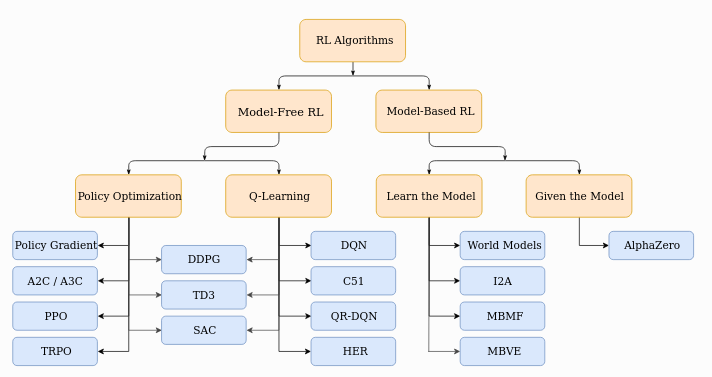
\includegraphics[width=0.7\textwidth]{images/rl_tree.png}
    \caption{RL Algorithm tree}
\end{figure}

We use the \textbf{P}roximal \textbf{P}olicy \textbf{O}ptimization (PPO) algorithm that is a very popular reinforcement learning algorithm that uses policy gradient to learn optimal policies and has a built in clipping mechanism that regulates how much the action-selection strategy can change over time. This generally results in the algorithm being stable during training.

\subsection{MAPPO}

For experiments using multiple snow plow agents we use a Mulit-Agent version of PP0 (MAPPO) used for cooperative mulit-agent objectives. In this case, plowing snow individually or collaboratively to gain the highest collective reward.


\section{Experiments}

\subsection{Experiment 1: 1-Agent + Full Observation}

\begin{table}[H]
    \centering
    \begin{tabular}{|c|c|}
        \hline
        \textbf{Parameter} & \textbf{Value} \\\hline
        Number of plows    & 1              \\\hline
        Observation        & FULL           \\\hline
        Algorithm          & PPO            \\\hline
        Recurrent          & False          \\\hline
        Road network       & network\_1     \\\hline
    \end{tabular}
    \caption{Experiment 1 parameters}
    \label{tab:exp1}
\end{table}

For the environment size in the first experiment we considered a grid of size $10 \times 19$ with 1 snow plow.

This experiment is meant to show the capabilities of one agent moving around the environment in an attempt to clear snow with full observability of the environment. With fill knowledge about the location of snow cells the agent should eventually after training have no problem navigating to find snow cells and



\subsection{Experiment 2: 1-Agent + Partial Observation}
\begin{table}[H]
    \centering
    \begin{tabular}{|c|c|}
        \hline
        \textbf{Parameter} & \textbf{Value}                   \\\hline
        Number of plows    & 1                                \\\hline
        Observation        & FULL                             \\\hline
        Algorithm          & PPO                              \\\hline
        Recurrent          & False                            \\\hline
        Road network       & network\_1                       \\\hline
        PO-range           & $(3 \times 3)$ or $(5 \times 5)$ \\\hline
    \end{tabular}
    \caption{Experiment 2 parameters}
    \label{tab:exp2}
\end{table}

% PO-range: $(3 \times 3)$ or $(5 \times 5)$

\subsection{Experiment 3: 2-Agents + Full Observation}
\begin{table}[H]
    \centering
    \begin{tabular}{|c|c|}
        \hline
        \textbf{Parameter} & \textbf{Value} \\\hline
        Number of plows    & 5              \\\hline
        Observation        & FULL           \\\hline
        Algorithm          & MAPPO          \\\hline
        Recurrent          & False          \\\hline
        Road network       & network\_3     \\\hline
    \end{tabular}
    \caption{Experiment 3 parameters}
    \label{tab:exp3}
\end{table}


\subsection{Experiment 4: 2-Agents + Partial Observation}
\begin{table}[H]
    \centering
    \begin{tabular}{|c|c|}
        \hline
        \textbf{Parameter} & \textbf{Value}                   \\\hline
        Number of plows    & 5                                \\\hline
        Observation        & FULL                             \\\hline
        Algorithm          & MAPPO                            \\\hline
        Recurrent          & False                            \\\hline
        Road network       & network\_3                       \\\hline
        PO-range           & $(3 \times 3)$ or $(5 \times 5)$ \\\hline
    \end{tabular}
    \caption{Experiment 4 parameters}
    \label{tab:exp4}
\end{table}


\section{Results}

\subsection{Experiment 1}

\subsection{Experiment 2}

\subsection{Experiment 3}

\subsection{Experiment 4}

\section{Conclusion}

\section{Discussion}

Our hopes for introducing \verb|snow_levels| was that multi-agents would converge into a policy that tells them to collaborate on areas with more snow. But on the other hand they should also realize that it will not be optimal for all situations because working on \verb|snow_level = 1| will still only give them +1 reward. Therefore, if they only observe level 1 cells, they would be encouraged to spread out more and cover more surface by themselves which would earn a higher total reward than doing it together all the time. This would simulate a work by demand  scenario that also commonly occurs in a realistic setting.

One potential shortcoming with this environment design might be that the decision-making strategy is not strongly motivated enough by the magnitude of the time steps that it takes to clear snow in relation to the reward they are getting. For example, will one agent "give up" chasing snow cells and turn around to help another agent that "in theory" would yield a higher reward? These dynamics might not be sufficiently expressed but could potentially be improved by adding more snow levels with linear or exponential time steps needed for clearing snow. However, this would probably also increase training time.




% =========== REFERENCES =========== 

\bibliographystyle{ieeetr}
\bibliography{rl}

\end{document}